\chapter{Uso de application launcher}
\begin{center}
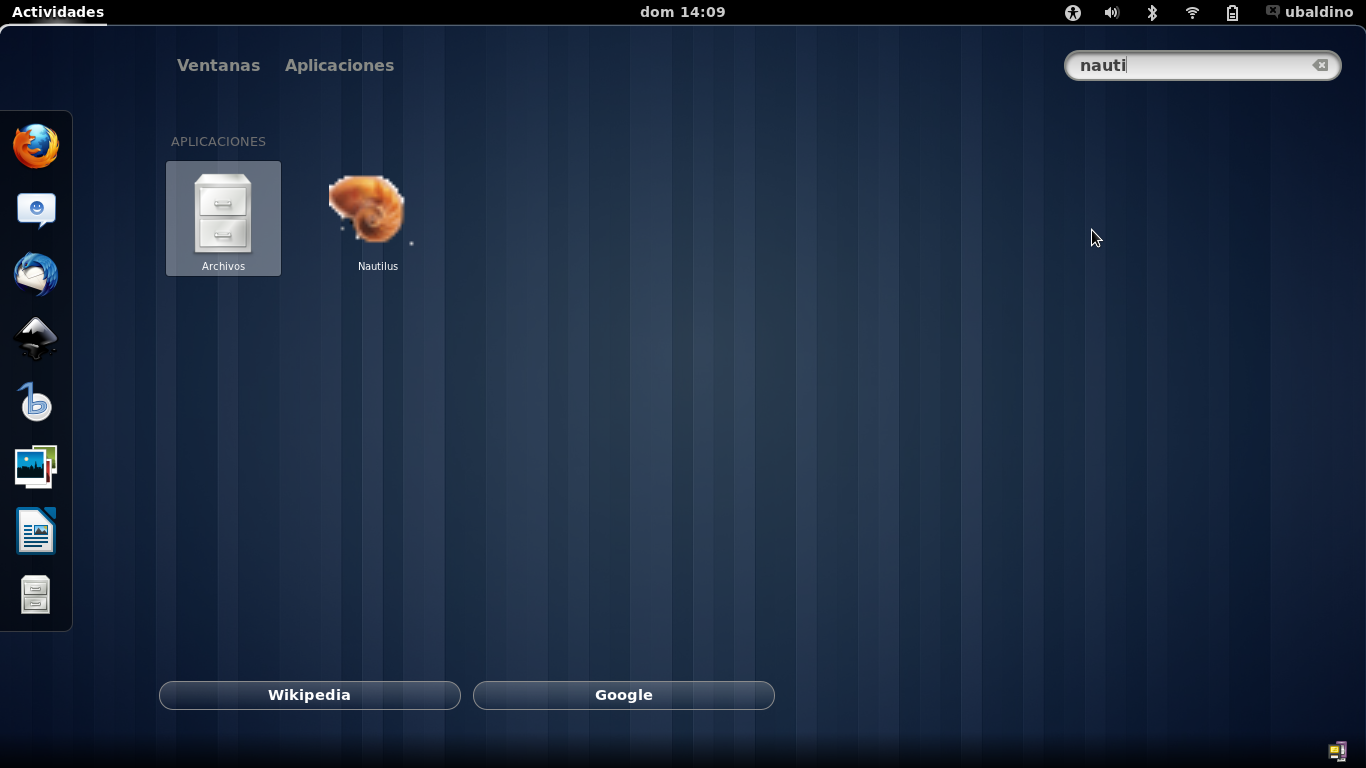
\includegraphics[scale=0.35]{gnome/Pantallazo9.png} 
\end{center}
En este capitulo aprenderemos la forma mas rápida de iniciar aplicaciones\\

Mueva el puntero de su ratón a la esquina de Actividades en la parte superior izquierda de la pantalla para mostrar la Vista de actividades. Aquí es donde puede encontrar todas sus aplicaciones. (También puede abrir la vista pulsando la supertecla o tecla windows.)
Hay distintas maneras de abrir una aplicación una vez que está en la vista de actividades:


\begin{itemize}
\item Comience a escribir las primeras letras de una aplicación; y la búsqueda comenzará al instante. (Si esto no sucede, pulse en la barra de búsqueda en la parte superior derecha de la pantalla y comience a escribir.) Pulse en el icono de la aplicación para iniciarla.
\item Pulse en la cabecera de Aplicaciones en la parte superior de la pantalla para ver una lista de aplicaciones que puede ejecutar. Puede filtrar por tipo, usando las categorías de la derecha, o buscar mediante la barra de búsqueda en la parte superior derecha. Pulse en el icono de la aplicación para iniciarla.
\item Puede iniciar una aplicación en un área de trabajo independiente arrastrando el icono de la aplicación desde el tablero (o desde la lista de aplicaciones), y colocándolo en una de las áreas de trabajo en la parte derecha de la pantalla. La aplicación se abrirá en el área de trabajo que elija.
\end{itemize}
Por ejemplo, para lanzar el gestor de archivos, escriba “nautilus” (sin las comillas). El nombre de la aplicación es el comando para lanzar el programa.\\

Algunas aplicaciones tienen iconos en el tablero, la franja vertical de los iconos en el lado izquierdo de la vista de actividades. Pulse en uno de ellos para iniciar la aplicación correspondiente.\\
Si tiene aplicaciones que usa muy frecuentemente, puede añadirlas al tablero.
\begin{center}
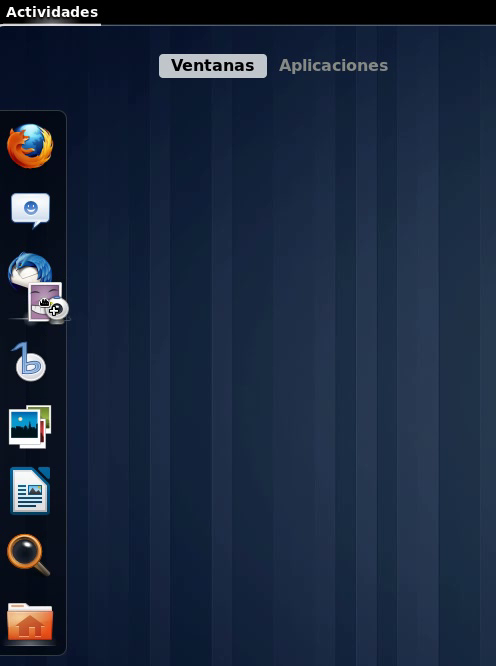
\includegraphics[scale=0.6]{gnome/aapli.png}
\end{center}